\documentclass[12pt,a4paper]{article}
\usepackage[utf8]{inputenc}
\usepackage{geometry}
\geometry{left=25mm,right=25mm,top=25mm,bottom=25mm}
\usepackage{times}
\usepackage{amsmath,amssymb}
\usepackage{graphicx}
\usepackage{caption}
\usepackage{subcaption}
\usepackage{booktabs}
\usepackage{multicol}
\usepackage{float}
\usepackage{hyperref}
\usepackage{tikz}
\usetikzlibrary{shapes.geometric, arrows.meta, positioning}
\usepackage{pgfplots}
\pgfplotsset{compat=1.17}

\title{Intelligent Condition Based Monitoring Using
Acoustic Signals for Air Compressors\\
\vspace{6pt}
\large A concise report based on Verma \textit{et al.}, IEEE Trans. on Reliability (2016)}
\author{Srinjoy Chakraborty}
\date{\today}
\begin{document} % <-- must come first
\maketitle % generates the title
\newpage
\tableofcontents % table of contents
\listoffigures % table of figures
\newpage
\begin{multicols}{2}
\section{Abstract}
\textit{Early detection of machine faults is vital to prevent costly downtime and ensure workplace safety. This paper presents a practical, data-driven process for building acoustic-based fault-diagnosis systems for reciprocating air compressors. The proposed pipeline is deliberately end-to-end: it covers how to collect acoustic data, how to choose the best microphone location, how to clean and normalize the recordings, which time/frequency/time–frequency features to extract, how to pick a compact yet informative feature set, and how to train and evaluate classifiers for multi-state fault recognition using SVM.
Overall, the paper demonstrates that a carefully designed acoustic monitoring pipeline can accurately and efficiently detect multiple fault modes using only one sensor location, making the approach attractive for cost-sensitive condition-based maintenance deployments main experimental paper used as the source is \cite{Verma2016}.}


\section{Introduction}
Rotating and reciprocating machines (compressors, motors, pumps) often show early warning signs in the form of acoustic or vibration signatures. Detecting faults early avoids costly downtime and safety hazards. Intelligent Condition-based monitoring (ICBM) aims to recognize incipient faults from sensory streams (acoustics, vibration, temperature, etc.) and thereby trigger maintenance before catastrophic failure. Acoustic measurements are especially attractive because they are typically easy to install and are relatively less sensitive to structural resonances compared to vibration sensors; however, acoustic recordings are often noisy and non-stationary, which makes automated analysis challenging.

Intelligent Condition-based monitoring (ICBM) is increasingly adopted in industry to detect early signs of machine degradation and to schedule maintenance before costly failures occur. Acoustic monitoring in particular is attractive for many rotating and reciprocating machines because microphones are inexpensive, simple to deploy, and can capture fault-related signatures that are often complementary to vibration and electrical measurements. However, practical acoustic monitoring faces two recurring challenges: (1) recordings are frequently contaminated by environmental and operational noise, and (2) signal characteristics are non-stationary and may vary across sensor locations. These issues make it difficult to select robust sensor placements and to extract consistently informative features for automated fault diagnosis.

A frequently overlooked but critical stage in the monitoring pipeline is \emph{Sensitive Position Analysis} (SPA) — the process of identifying where on the machine a sensor should be mounted to maximize fault detectability. Traditional SPA methods rely on straightforward statistics (e.g., RMS, peak, variance) and on simple cross-correlation to avoid redundant locations. While effective in quiet and controlled settings, these techniques can fail when recordings are influenced by heterogeneous noise or transient disturbances. To make SPA robust in such realistic settings, a preprocessing approach that can separate meaningful signal components from noise — and do so adaptively for non-stationary signals — is required.

This study proposes an end-to-end, data-driven pipeline that addresses these challenges. The core idea is to combine Empirical Mode Decomposition (EMD) with conventional preprocessing, feature extraction, and principled feature selection so that SPA and subsequent classification operate on cleaner, more informative representations. EMD adaptively decomposes each recording into intrinsic mode functions (IMFs). By selecting IMFs that exhibit strong relevance to the recorded waveform (and discarding IMFs dominated by noise or numerical artifacts), we reconstruct a denoised version of the acoustic signal. Computing the Hilbert envelope of this reconstructed signal and deriving compact statistics (RMS and absolute mean) provides stable ranking criteria that are less sensitive to transients and background noise. The remainder of the pipeline extracts a broad set of time, frequency, and time–frequency features, uses mutual-information and other feature-selection techniques to obtain a compact descriptor set, and employs multiclass SVMs for state recognition.

The proposed approach is validated on a real single-stage reciprocating air compressor with eight distinct operating states (one healthy state and seven seeded faults). Key practical choices made in the study include a robust clipping/segment-selection strategy to avoid transients, a normalization routine that mitigates the influence of extreme samples, and an empirical selection of correlation thresholds for choosing relevant IMFs. Experiments demonstrate that, using recordings from a single optimally chosen microphone position, the pipeline reliably distinguishes the seeded faults and achieves high classification accuracy while keeping computational overhead manageable.

The main contributions of this work can be summarized as follows:
\begin{itemize}
  \item An \textbf{EMD-based SPA} procedure that improves the robustness of sensor-position ranking under noisy and non-stationary conditions by reconstructing signals from relevant IMFs and using their Hilbert envelopes for ranking.
  \item A practical, reproducible DAQ and preprocessing protocol (filtering, clipping, smoothing, and robust normalization) that yields stable input for decomposition and feature extraction.
  \item A comprehensive evaluation on a real compressor testbed showing that a compact feature set—selected via mutual-information-based techniques—combined with multiclass SVMs, can accurately identify multiple fault modes from a single microphone location.
\end{itemize}
\end{multicols}
\begin{figure}[H]
    \centering
    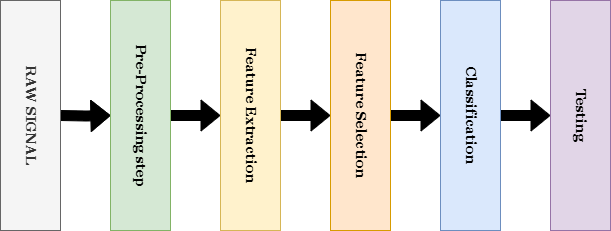
\includegraphics[width=1\linewidth]{Diagrams/icbmintro.drawio.png}
    \caption{System Architecture}
    \label{fig:sysarch}
\end{figure}
\begin{multicols}{2}

The above diagram ~\ref{fig:sysarch} shows the overall system architecture. The flow contains 6 steps (1) Data Acquisition using microphones $\rightarrow$ Raw Signal, (2) Pre-processing, (3) Feature Extraction, (4) Feature Selection, (5) Classification $\rightarrow$ SVM, (6) Testing and Validation.
The rest of this report is organized as follows. Section~\ref{sec:daq} describes the data acquisition setup and recording protocol. Section~\ref{sec:preprocess} summarizes the preprocessing steps used prior to decomposition. Section~\ref{sec:features} outlines the feature extraction and selection methods, and Section~\ref{sec:classification} describes the classification strategy. Experimental results and analysis are reported in Section~\ref{sec:results}, followed by conclusions and directions for future work in Section~\ref{sec:conclusion}. The DAQ setup and specific implementation details follow the experimental design in \cite{Verma2016}.

\section{Data Acquisition (DAQ) System}
\label{sec:daq}

This study used acoustic recordings to capture machine condition signatures. The DAQ choices focused on reproducibility and on maximizing signal quality while keeping the setup simple.

\subsection{Hardware and placement}
\begin{itemize}
  \item \textbf{Microphones:} Unidirectional microphones were used to preferentially pick up sound directed toward each sensor and to reduce off-axis ambient noise.
  \item \textbf{DAQ hardware:} Recordings were acquired using a National Instruments NI-9234 dynamic signal acquisition module (four channels, 24-bit) connected via an NI-9172 chassis to a PC running LabVIEW for capture and storage. This setup allows up to four simultaneous microphone channels at high sample rates.
  \item \textbf{Sensor distance:} Empirical tests showed the cleanest and loudest captures when the microphone was placed approximately 1.5 cm from the machine surface; this distance was used consistently for all recordings.
\end{itemize}
\subsection{Recording procedure}
\begin{itemize}
  \item \textbf{Duration \& sampling:} Each recording is 5 seconds long sampled at 50 kHz and stored as 24-bit PCM. Thus each raw file contains 250,000 samples.
  \item \textbf{Candidate positions:} To perform Sensitive Position Analysis (SPA) the machine was sampled at multiple candidate locations (the original study used 24 positions) so that a robust ranking of sensor positions could be obtained.
\end{itemize}
\subsubsection{Preliminary observations}
Practical tests revealed:
\begin{itemize}
    \item Microphones placed at roughly {1.5}{cm} from the machine provided stronger signals and reduced background contamination.
    \item Acoustic useful content predominantly lies below {12}{kHz} for the compressor under study \cite{Verma2016}; therefore, pre-processing included a high-pass filter (to remove fan hum) and a low-pass filter at {12}{kHz}.
    \item A clipping strategy (segment selection) with overlap helps to choose the most stable portion of each recording for robust analysis (detailed in Section~\ref{sec:preprocess}).
\end{itemize}
\section{Pre-Processing}
\label{sec:preprocess}
\begin{itemize}
  \item \textbf{Useful bandwidth:} For this compressor, the informative acoustic content lies largely below 12 kHz; accordingly, later processing uses a low-pass cutoff around 12 kHz and a high-pass ``fan'' filter near 400 Hz to remove known background hums/noises.
  \item \textbf{Clipping} Each 5 s recording is split into 9, 1 s segments with 50\% overlap; the segment with the minimum standard deviation is selected for analysis to avoid transient spikes and to choose the most stable portion of the recording.
  \item \textbf{Smoothing \& normalization:} A simple moving-average smoother removes impulsive outliers, and a robust min–max style normalization (ignore 0.025\% extreme samples at both tails when computing min/max) is used so that scaling is not driven by rare outliers.
  \item \textbf{Storage \& labeling:} Store raw .dat (24-bit PCM) files to ensure later classification stages.
\end{itemize}
\begin{figure}[H]
    \centering
    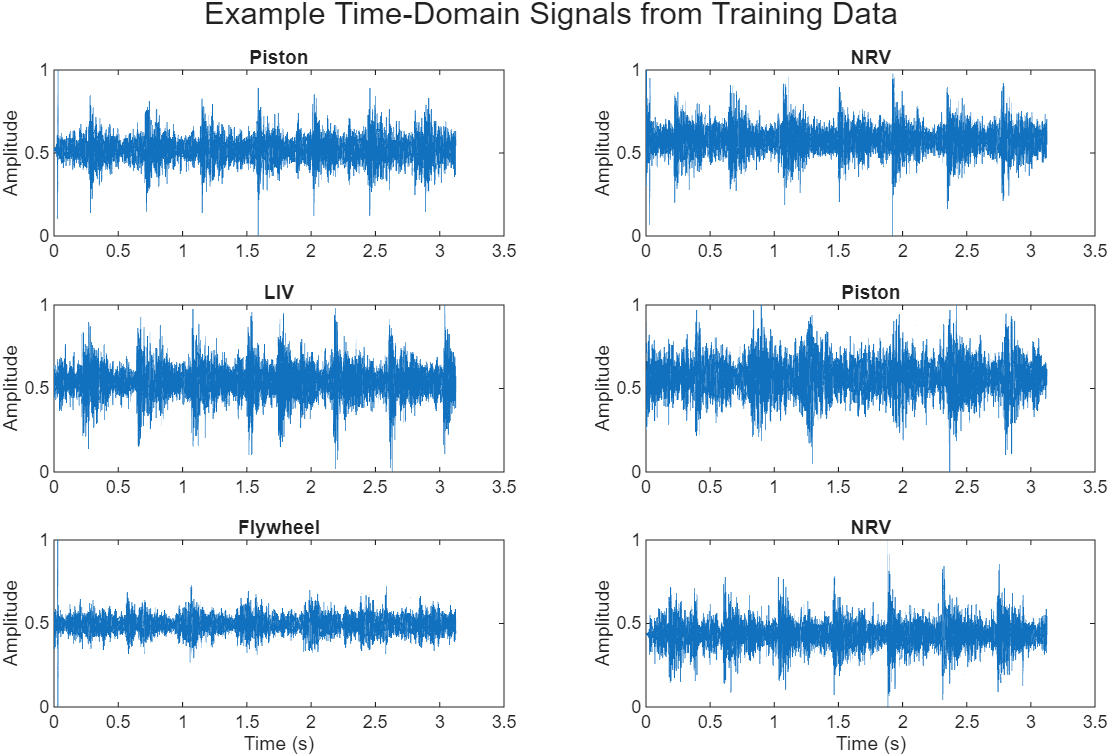
\includegraphics[width=1\linewidth]{Diagrams/preprocessing.png}
    \caption{Preprocessing steps}
    \label{fig:preprocessing steps}
\end{figure}
\section{Feature Extraction}
\subsection{1.}
\subsection{2.}
\subsection{3.}
\section{Feature Selection}
\label{sec:features}
Principal Component Analysis (PCA) is a dimensionality reduction technique that
transforms a large set of correlated features into a smaller set of uncorrelated
variables, known as principal components. Each component is an orthogonal
projection of the original features and is ranked according to the variance it
captures from the dataset. This allows redundant and less informative features
to be compressed into a compact representation while still retaining the
dominant structure of the data.

In the context of acoustic fault diagnosis, where hundreds of features are
extracted across time, frequency, and wavelet domains, directly using the full
feature set increases computational burden and may reduce classifier performance
due to redundancy. To address this, we apply PCA to the $286$-dimensional feature
vectors, standardize them, and project them into a lower-dimensional subspace.
The number of retained components was varied (from 10 to 200) to evaluate the
trade-off between dimensionality and classification accuracy. These principal
components were then used as inputs to the Support Vector Machine (SVM)
classifiers under both One-vs-All (OVA) and One-vs-One (OVO) schemes. This
approach ensures faster computation, reduces overfitting, and maintains the
ability to distinguish between healthy and faulty compressor states.
\begin{figure}[H]
    \centering
    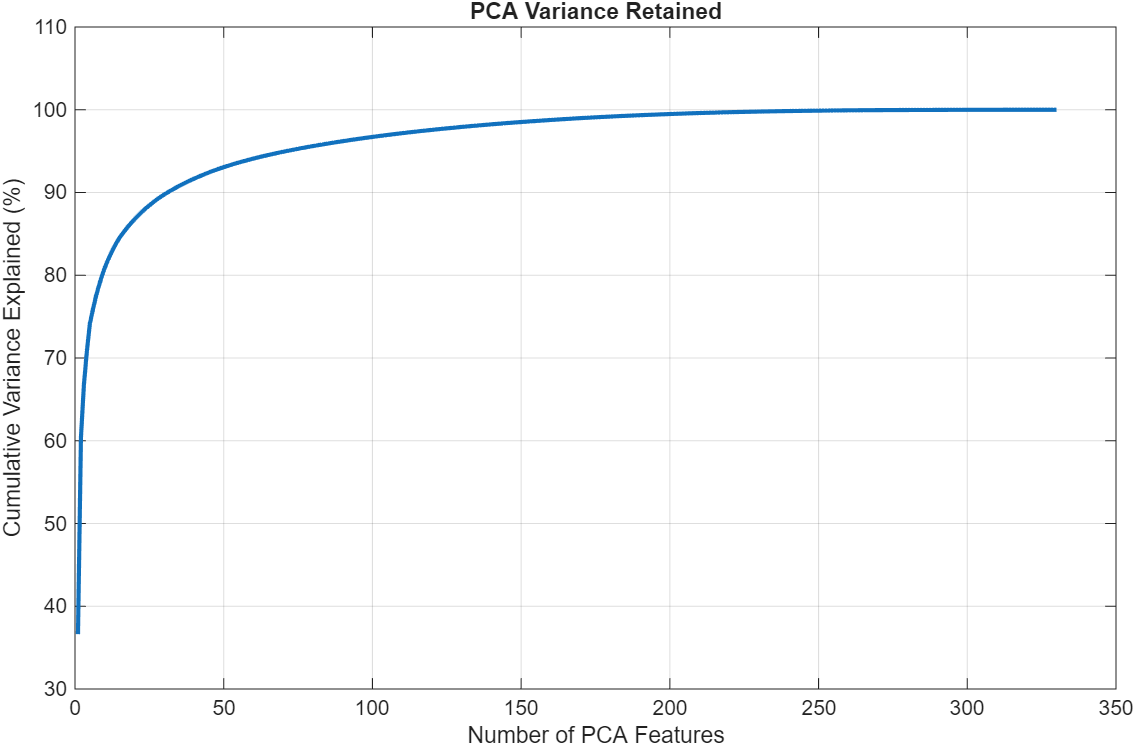
\includegraphics[width=1\linewidth]{Diagrams/pcavar.png}
    \caption{PCA Variance}
    \label{fig:PCA Variance}
\end{figure}
\section{Use Case}
\subsection{Classes, labels and Test-Train Split}
\begin{figure}[H]
    \centering
    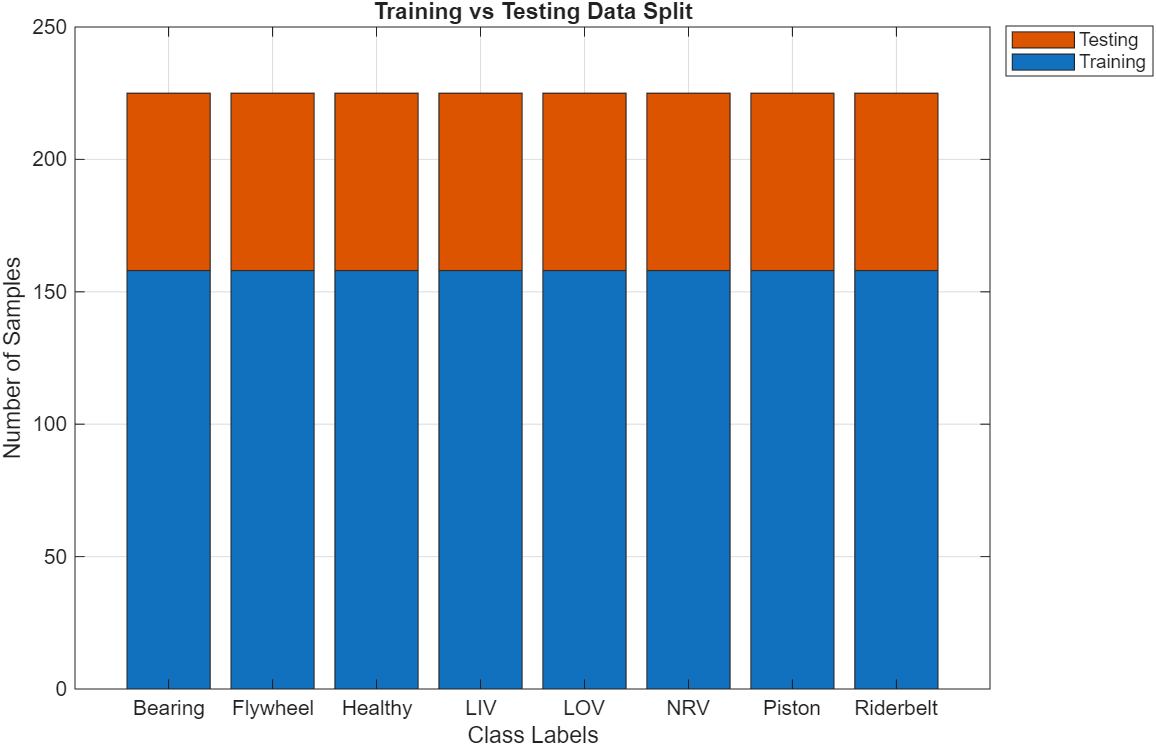
\includegraphics[width=1\linewidth]{Diagrams/split.png}
    \caption{test train split}
    \label{fig:split}
\end{figure}
\subsection{techniques used}
\subsection{SVM}
\label{sec:classification}
\section{Results}
\label{sec:results}
\begin{figure}[H]
    \centering
    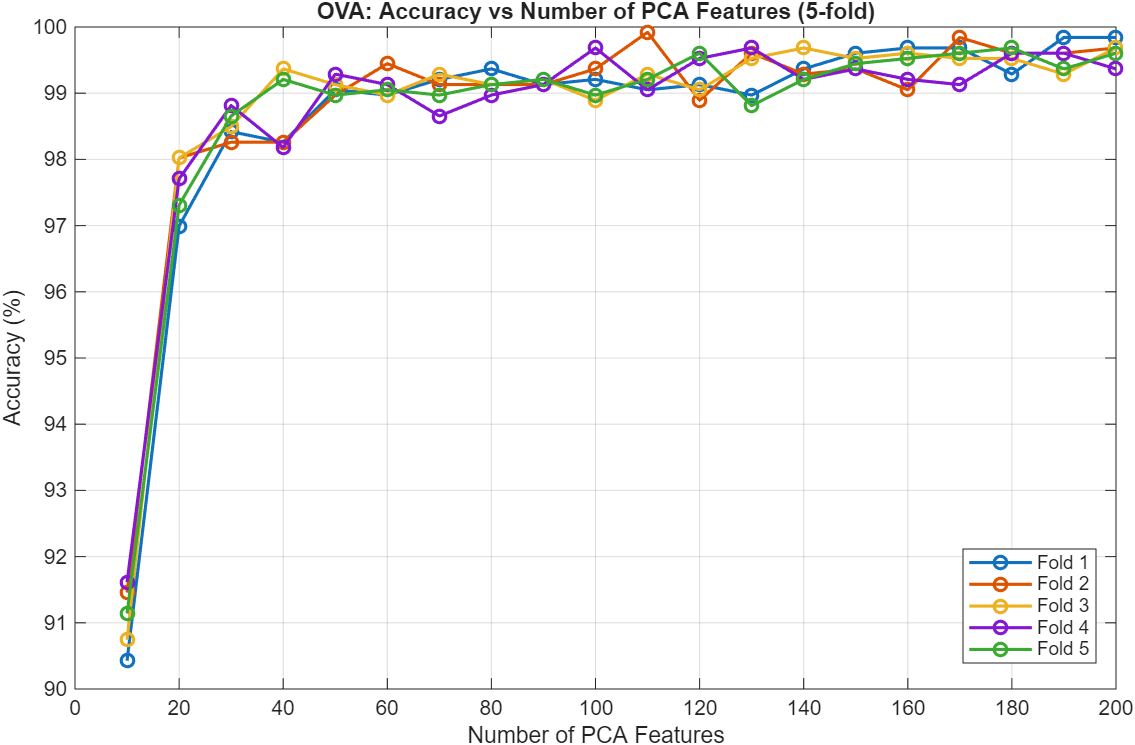
\includegraphics[width=1\linewidth]{Diagrams/res1.png}
    \caption{OVA result}
    \label{fig:ova}
\end{figure}
\begin{figure}[H]
    \centering
    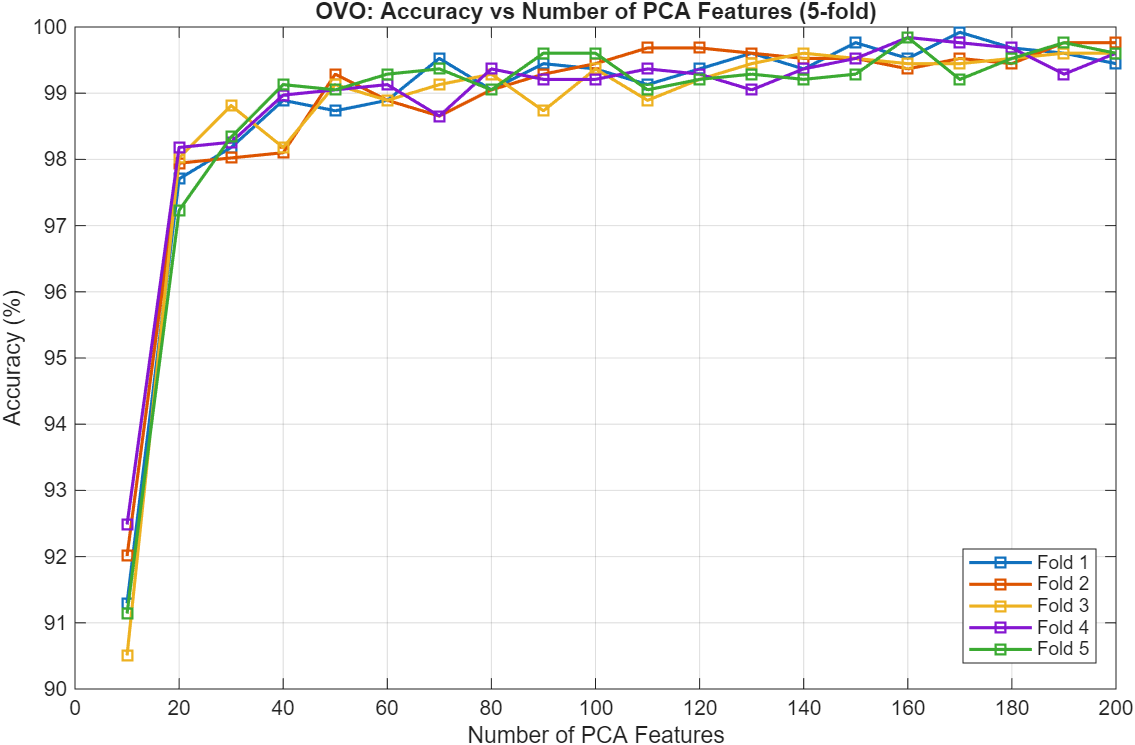
\includegraphics[width=1\linewidth]{Diagrams/res2.png}
    \caption{OVO result}
    \label{fig:ovo}
\end{figure}
\section{Conclusion}
\label{sec:conclusion}
\section*{References}
\begin{thebibliography}{1}
\bibitem{Verma2016}
N.~K. Verma, R.~K. Sevakula, S.~Dixit, and A.~Salour, ``Intelligent condition based monitoring using acoustic signals for air compressors,'' \emph{IEEE Transactions on Reliability}, vol.~65, no.~1, pp. 291--307, Mar. 2016. doi:10.1109/TR.2015.2459684.
\end{thebibliography}
\end{multicols}
\end{document}
